\documentclass{article}
\usepackage[utf8]{inputenc}
\usepackage[T1]{fontenc}
\usepackage[italian]{babel}
\usepackage{geometry}
\usepackage{graphicx}
\usepackage{amsmath}
\usepackage[section]{placeins} % <--- LA SOLUZIONE DEFINITIVA

\geometry{a4paper, margin=1in}

\title{Capitolo 4 - Crittografia Asimmetrica e Funzioni Hash}
\author{}
\date{}

\begin{document}
\maketitle

\section{Le Firme Digitali (Digital Signatures)}
Mentre la cifratura standard serve a nascondere il contenuto di un messaggio, la firma digitale serve a certificarne la provenienza e l'integrità. Secondo lo standard NIST FIPS PUB 186-4, \textit{una firma digitale è il risultato di una trasformazione crittografica che fornisce l'autenticazione dell'origine, garantisce l'integrità dei dati e assicura il "non ripudio" (ovvero, il mittente non può negare di aver inviato quel messaggio)}. È fondamentale sottolineare che la firma digitale, di per sé, non fornisce alcuna confidenzialità: il messaggio firmato può viaggiare "in chiaro" ed essere letto da chiunque.

A livello operativo, la firma sfrutta la crittografia asimmetrica al contrario rispetto alla cifratura classica. Il mittente (Bob) calcola un hash del proprio messaggio e lo cifra utilizzando la propria \textbf{chiave privata}. Questo blocco cifrato viene allegato al messaggio come "firma". Quando il destinatario (Alice) riceve il pacchetto, utilizza la \textbf{chiave pubblica} di Bob per decifrare la firma e confronta l'hash ottenuto con quello calcolato autonomamente sul messaggio ricevuto. Se i due hash coincidono, la firma è valida. Tra gli algoritmi standard più utilizzati per questa operazione troviamo il DSA (Digital Signature Algorithm), l'RSA e l'ECDSA (basato sulle curve ellittiche).

% Usiamo [htbp] per riempire i buchi bianchi col testo, 
% ma placeins bloccherà l'immagine prima della prossima \section
\begin{figure}[htbp] 
     \centering
     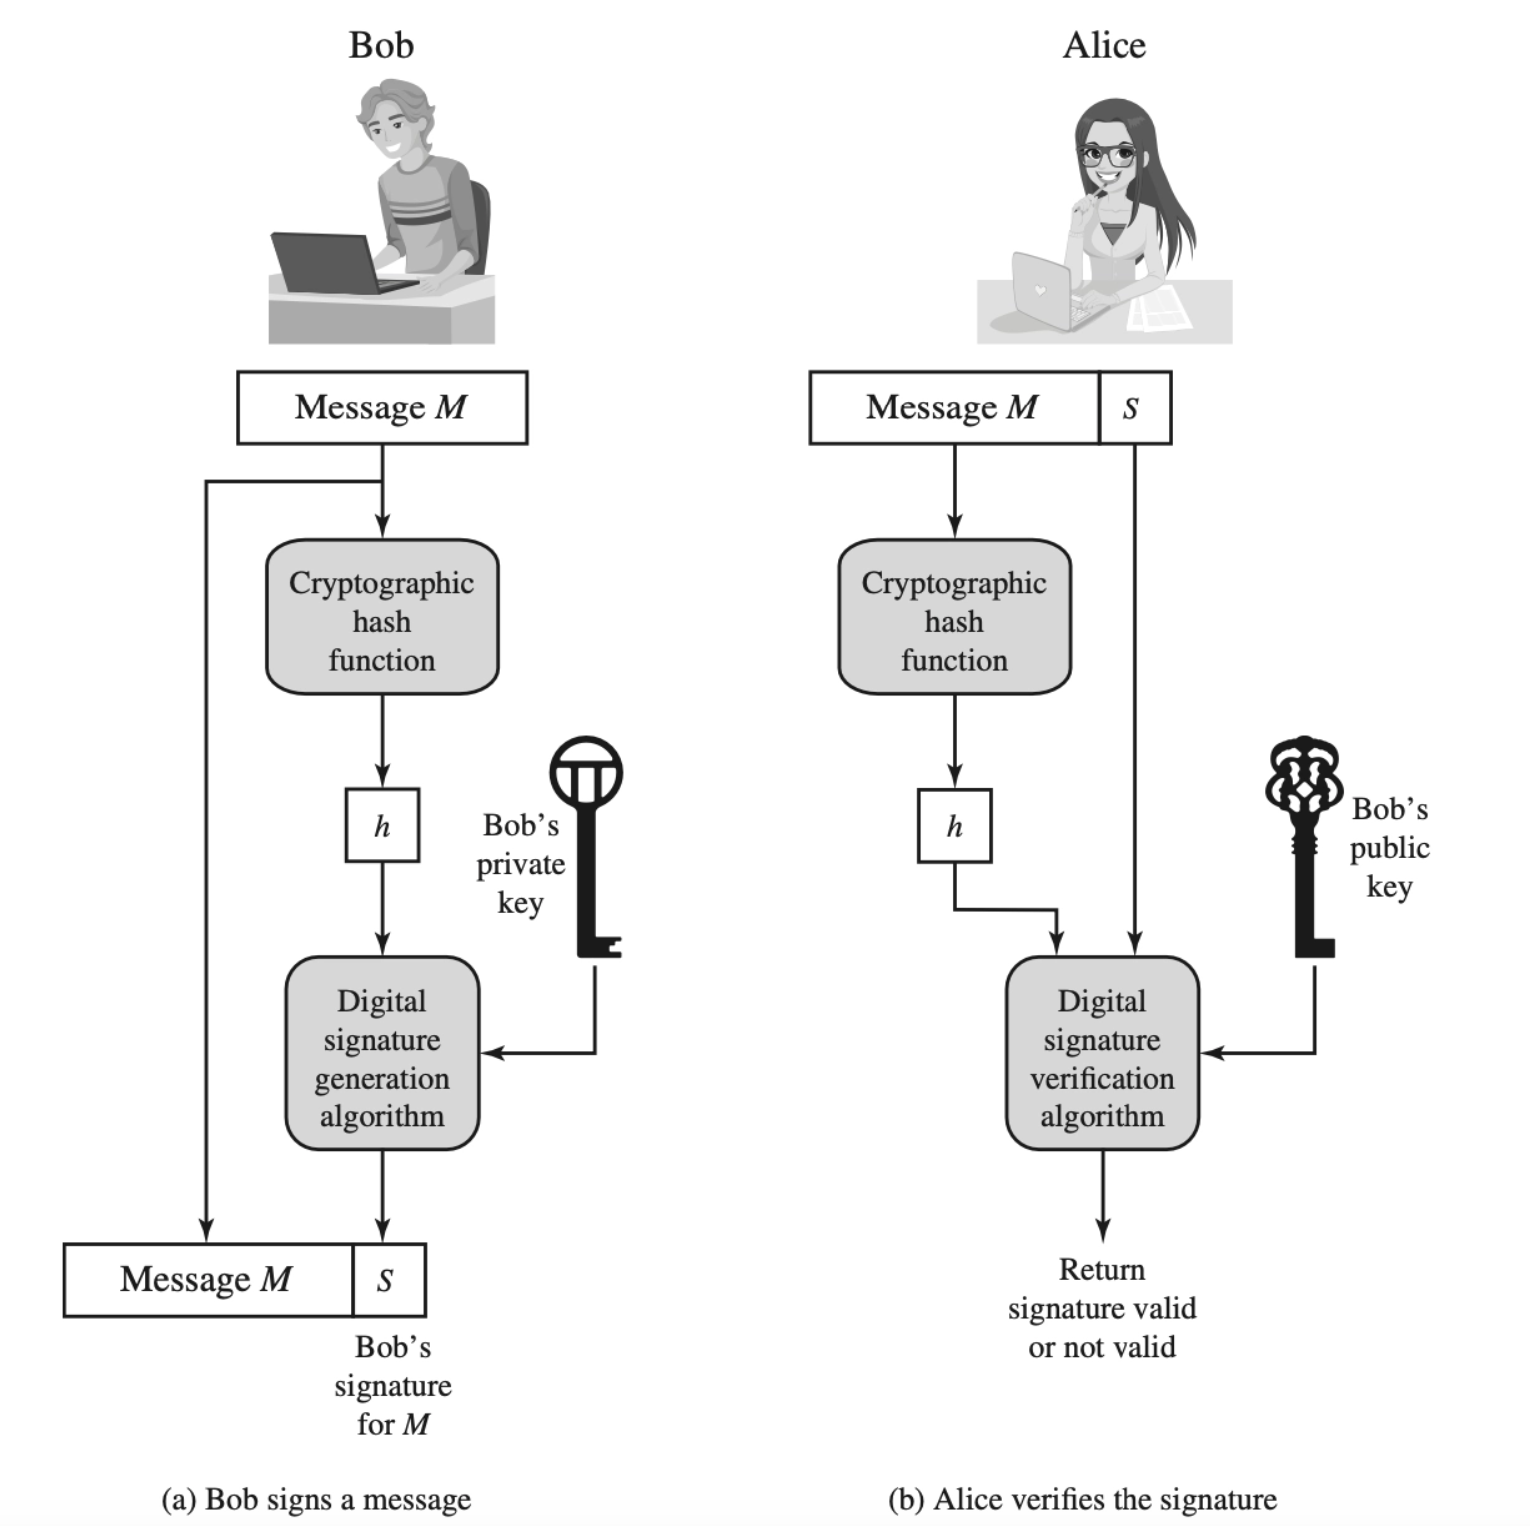
\includegraphics[width=0.8\textwidth]{Screenshot 2026-05-30 alle 16.26.57.png}
     \caption{Schema della generazione e verifica della firma digitale}
 \end{figure}


\section{La Vulnerabilità dell'Identità e i Certificati Digitali}
Il sistema delle firme digitali (e della crittografia asimmetrica in generale) poggia su un assunto pericoloso: la chiave pubblica è, per l'appunto, pubblica. Il difetto critico di questo schema è che un attaccante potrebbe creare una propria coppia di chiavi, diffondere la chiave pubblica spacciandosi per Bob e intercettare i messaggi a lui destinati, oppure inviare messaggi falsamente firmati a suo nome.

La soluzione universale a questo problema di "fiducia" è il \textbf{Certificato a Chiave Pubblica}. Il certificato funge da carta d'identità digitale: è un documento che lega in modo indissolubile l'identità di un utente (User ID) alla sua specifica chiave pubblica. A garantire la veridicità di questo legame interviene una terza parte fidata, chiamata \textbf{Certification Authority (CA)} (come Aruba, InfoCert o enti governativi), la quale si fa garante dell'identità dell'utente. Lo fa emettendo un Certificato Digitale all'interno del quale i dati anagrafici dell'utente vengono vincolati matematicamente alla sua chiave pubblica. Per rendere questo documento inalterabile, la CA lo sigilla apponendovi la propria firma digitale, calcolata utilizzando la sua chiave privata.

Il processo di certificazione è rigoroso: l'utente genera la propria coppia di chiavi e invia la chiave pubblica e i propri dati alla CA. La CA verifica l'identità dell'utente, impacchetta i dati, aggiunge un periodo di validità e calcola l'hash di questo blocco. Infine, la CA firma il certificato cifrando l'hash con la propria \textbf{chiave privata}. Quando Alice riceve il certificato di Bob, le basterà utilizzare la chiave pubblica della CA (che è universalmente nota e preinstallata nei sistemi operativi) per verificare la firma della CA stessa; se la firma è valida, Alice ha la certezza matematica che la chiave pubblica contenuta in quel certificato appartiene veramente a Bob.

\begin{figure}[htbp]
     \centering
     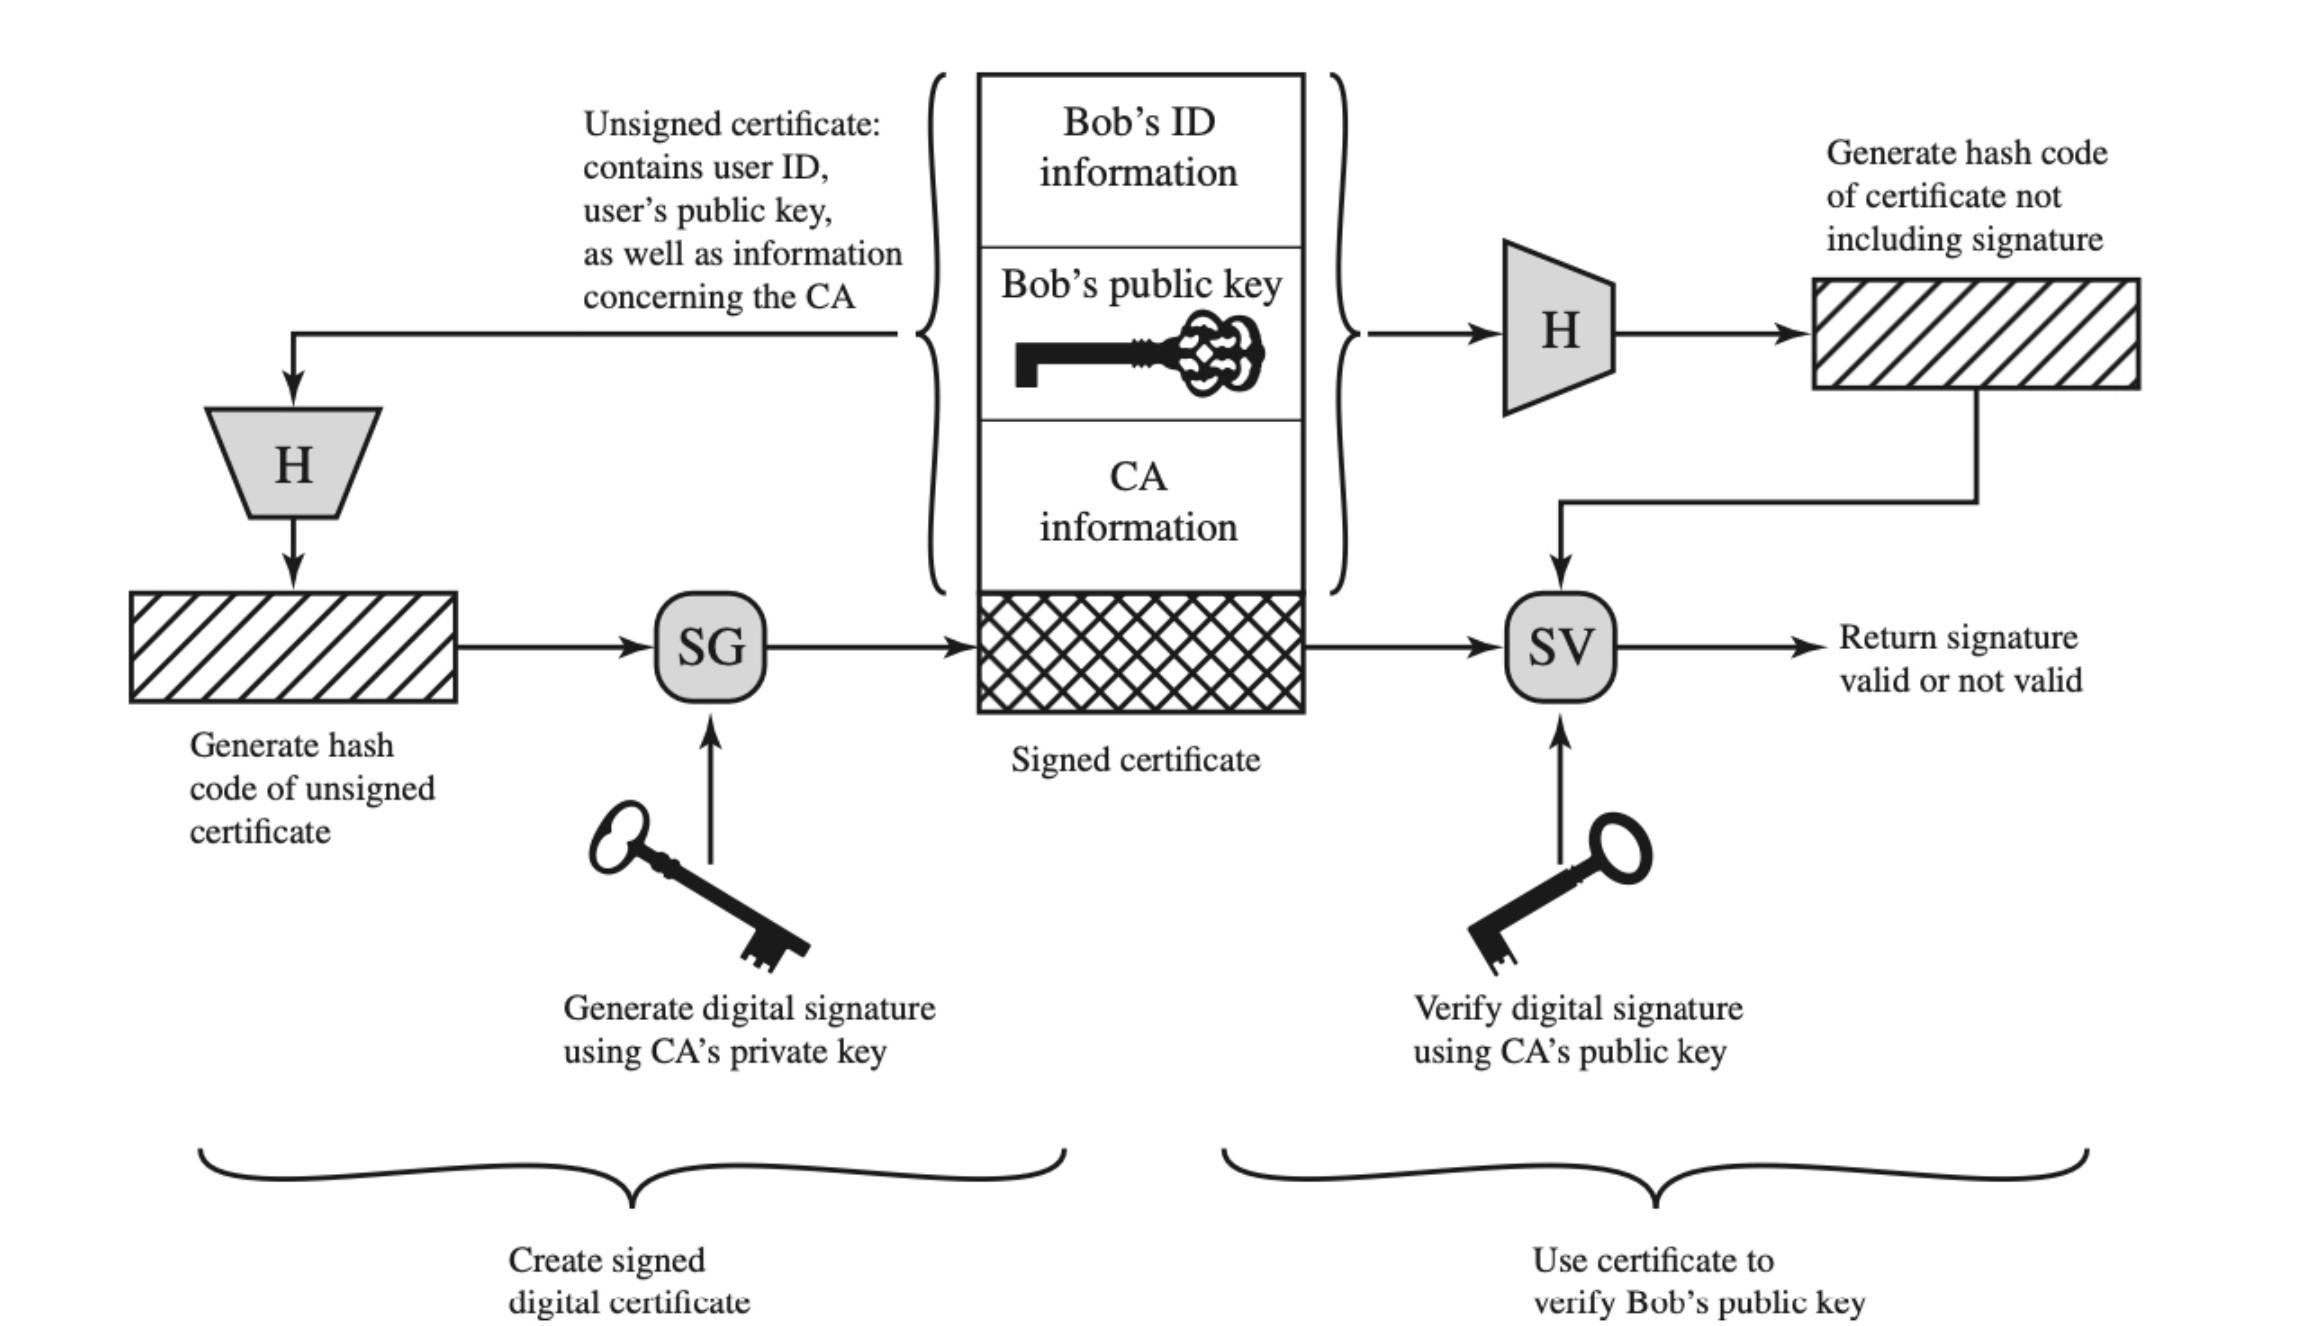
\includegraphics[width=0.8\textwidth]{Screenshot 2026-05-30 alle 16.26.19.png}
     \caption{Processo di creazione e verifica di un certificato firmato}
 \end{figure}


\section{Le Buste Digitali (Digital Envelopes)}
La crittografia a chiave pubblica è estremamente sicura, ma è troppo lenta e computazionalmente pesante per cifrare grossi volumi di dati. D'altra parte, la crittografia simmetrica è velocissima, ma richiede che mittente e destinatario si siano già scambiati una chiave segreta in modo sicuro. La \textbf{Busta Digitale (Digital Envelope)} unisce il meglio di questi due mondi per permettere a due entità di comunicare in modo confidenziale senza essersi mai accordate prima.

Il processo funziona come un sistema ibrido. Quando Bob vuole inviare un grosso file segreto ad Alice, il suo sistema genera istantaneamente una chiave simmetrica casuale e monouso (One-time key). Il file viene cifrato rapidamente con questa chiave simmetrica. A questo punto, per far arrivare la chiave simmetrica ad Alice in sicurezza, Bob la cifra utilizzando la \textbf{chiave pubblica di Alice} (creando così la "busta digitale"). I due pacchetti (il file cifrato simmetricamente e la chiave cifrata asimmetricamente) vengono inviati insieme. Alice, ricevuta la trasmissione, utilizzerà la propria chiave privata per "aprire la busta", estrarre la chiave simmetrica monouso e usarla per decifrare l'intero messaggio in modo rapido e sicuro.

\begin{figure}[htbp]
     \centering
     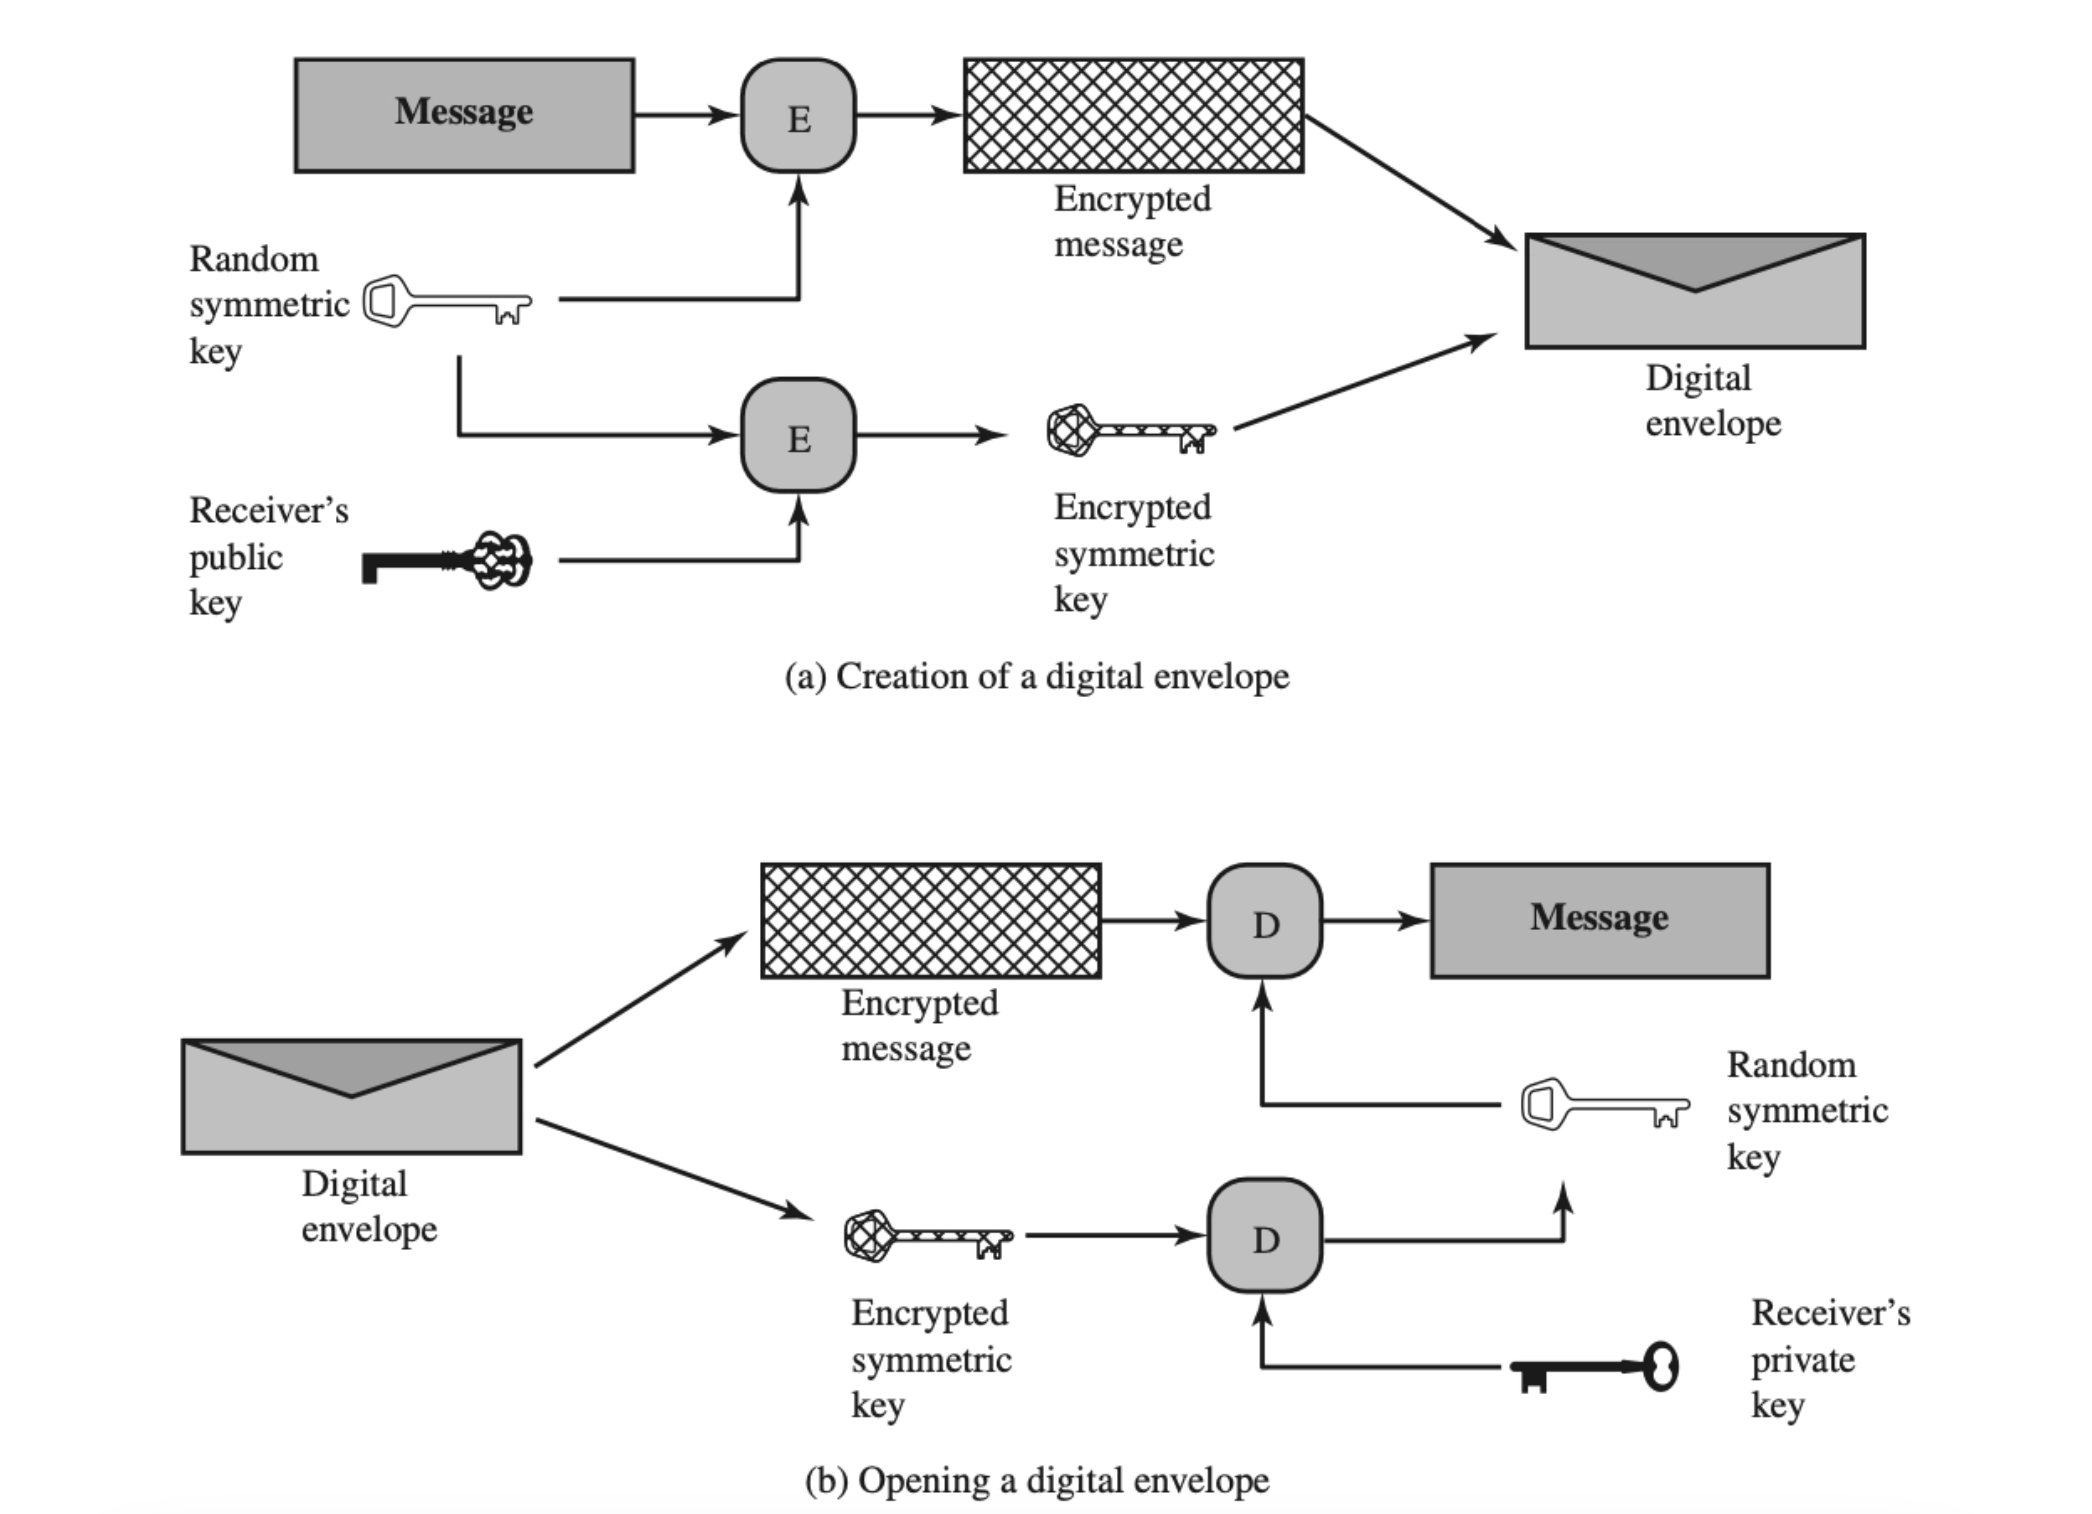
\includegraphics[width=0.8\textwidth]{Screenshot 2026-05-30 alle 16.26.29.png}
     \caption{Creazione e apertura di una busta digitale}
 \end{figure}


\section{Numeri Casuali e Pseudocasuali (RNG)}
Un elemento cardine che fa funzionare le buste digitali e innumerevoli altri meccanismi crittografici è la disponibilità di numeri casuali. Vengono utilizzati costantemente per generare chiavi di sessione temporanee, flussi di chiavi per cifrari a flusso e per le operazioni di \textit{handshaking} per prevenire gli attacchi di ripetizione (Replay attacks).

Per essere crittograficamente sicuro, un generatore deve rispettare requisiti severi. I numeri prodotti devono superare test di \textbf{Casualità} statistica (avere una distribuzione uniforme in cui ogni numero ha la stessa probabilità di uscire) e di \textbf{Indipendenza} (nessun valore deve poter essere dedotto analizzando i valori precedenti o successivi). Soprattutto, la sequenza deve essere caratterizzata da totale \textbf{Imprevedibilità}.

Esistono due approcci principali per ottenere questa entropia. I \textbf{Numeri Pseudocasuali (PRNG)} sono generati da algoritmi matematici deterministici; pur superando i test statistici di casualità, sono potenzialmente prevedibili se un attaccante riesce a scoprire il "seme" (seed) iniziale e l'algoritmo utilizzato. I veri e propri \textbf{Numeri Casuali (TRNG - True Random Number Generator)}, invece, abbandonano il determinismo matematico per estrarre la loro imprevedibilità direttamente dall'osservazione di processi fisici o naturali caotici, come il rumore termico dei circuiti elettronici o specifici effetti quantistici, garantendo una sicurezza assoluta contro la predizione.

\end{document}